\documentclass[letter, 10pt]{article}
\usepackage[utf8]{inputenc}
\usepackage[spanish]{babel}
\usepackage{amsfonts}
\usepackage{amsmath}
\usepackage{graphicx}
\usepackage{url}
\usepackage{hyperref}
\usepackage[top=3cm,bottom=3cm,left=3.5cm,right=3.5cm,footskip=1.5cm,headheight=1.5cm,headsep=.5cm,textheight=3cm]{geometry}


\begin{document}
\bibliographystyle{plain}
\pagestyle{empty}

\title{Taller de Modelos y Métodos Cuantitativos \\ \begin{Large}Estado del Arte: ``Car Sequencing Problem''\end{Large}}
\author{Cristián D. Maureira Fredes}
\date{\today}
\maketitle

\section{Introducción}
\label{sec:introduccion}
Una expresión regular,
a menudo llamada también patrón,
es una expresión que describe un conjunto de cadenas sin enumerar sus elementos.

Además,
normalmente representan otro grupo de caracteres mayor,
de tal forma que podemos comparar el patrón con otro conjunto de caracteres para ver las coincidencias.

La mayoría de las formalizaciones proporcionan los siguientes constructores:
una expresión regular es una forma de representar a los lenguajes regulares
(finitos o infinitos) y se construye utilizando caracteres del alfabeto
sobre el cual se define el lenguaje.

Específicamente,
las expresiones regulares se construyen utilizando los operadores
unión, concatenación y clausura de Kleene.

Las expresiones regulares en UNIX (RE's) están recogidas en el estándar POSIX 1003.2.



\section{Definición del Problema}
\label{sec:definicionProblema}
%Descripción del problema, su complejidad, en que consiste, cuales son sus objetivos,
%restricciones, variantes más conocidas. 

El \emph{Car Sequencing Problem} es un problema de satisfacción de restricciones (CSP), posee la
característica de ser NP-duro~\footnote{
NP-duro es el conjunto de los problemas de decisión que contiene los problemas H
tales que todo problema L en NP puede ser transformado polinomialmente en H.
Esta clase puede ser descrita como conteniendo los problemas de decisión que son
al menos tan difíciles como un problema de NP.}
, además corresponde a un tipo de variación del problema NP-completo \emph{Job-Shop Scheduling}.%,
%pero con un uso de razonamiento automatizado, es decir, con un enfoque dedicado a estudiar y comprender
%diferentes características del razonamiento, permitiendo así construir programas que le den la posibilidad
%a los computadores para razonar en forma autónoma.
 
Siguiendo la misma idea, es válido señalar que el \emph{Car Sequencing Problem} es un tipo de problema de planificación
de tareas en una línea de ensamblaje de autos, donde cada uno es perteneciente a un clase de automóvil, debido al conjunto
de opciones y accesorios que posee (airo acondicionado, centralizado eléctrico, etc), y cada una de las opciones o
accesorios se instala en una planta distinta, por lo que el objetivo principal es el poder encontrar el orden en la
secuencia de los vehículos, preocupándonos de no exceder la capacidad de cada planta de ensamblaje y también cumplir con la demanda.

Por lo tanto, si realizamos una definición más formal de nuestro problema, podríamos decir lo siguiente:
Teniendo una lista de vehículos dada, cada uno con sus respectivas opciones requeridas,
necesitamos establecer un orden en la línea de ensamblaje, con el fin de que cada subsecuencia de $q$ vehículos
tengamos a lo más $p$ que requieren de una determinada opción. Es importante tener en consideración que los
valores de $p$ y $q$ están asociados a cada opción de los vehículos.

Con respecto a la información que el problema otorga, podemos decir que contamos con:
\begin{itemize}
	\item Cantidad de vehículos de cada tipo o clase a producir (demanda)
	\item Lista de las opciones con la cual se constituye cada tipo o clase de vehículo, la cual puede utilizar una representación
		booleana para saber si cierto tipo de automóvil posee o no una determinada opción.
	\item Capacidad de las plantas que se preocupan de instalar la determinada opción.
\end{itemize}

Nuestro objetivo principal es:
\begin{itemize}
	\item Encontrar un orden en nuestra secuencia, que sirva para minimizar el costo por cada restricción insatisfecha.
\end{itemize}

Con respecto a las restricciones, tenemos que:
\begin{itemize}
	\item En cada subsecuencia de los $q$ vehículos, a lo más pueden haber $p$ que requieran de la opción determinada.
		Donde $p$ y $q$ son valores asociados a cada opción.
	\item La capacidad de cada planta de ensamblaje no puede ser excedida, es decir, cumplir con la demanda de cada automóvil
		sin abusar de una planta determinada.
	\item Por cada tipo de auto, el numero de autos de ese tipo debe ser secuenciado, es decir, todos los automóviles de cada clase
		deben estar presente en una secuencia determinada.
\end{itemize}





\subsection{Estado del arte problema}
\label{sec:estadoArte}
%En que nivel se ha investigado la técnica aplicada al problema
%     (existe o no investigación, cuantas, cuales modelos, componentes
%     de la técnica, como es su desempeño, etc.).
%     En caso de no existir investigación o si a usted le parece que es
%     un aporte, experiencias con problemas similares o que podría ser útil
%     para su trabajo.

%existe o no?
%experiencias similares
\frame
{
\frametitle{Estado del Arte}
\framesubtitle{Existencia del acercamiento}
\begin{itemize}
	\item Actualmente en las grandes fuentes de publicaciones, como lo son:
	\begin{itemize}
		\item ACM.
		\item Springerlink.
		\item IEEE.
		\item Google Scholar.
	\end{itemize}
	\item \textbf{NO} existe un acercamiento utilizando \emph{Clonal Selection}
		para la resolución del \emph{Car Sequencing Problem}.
	\item Estado del arte del \emph{ROADEF}.
\end{itemize}
}

\frame
{
\frametitle{Estado del Arte}
\framesubtitle{Experiencias Similares}
\begin{block}{Mobile Robot Path Planning}
\begin{itemize}
	\item Operadores Inmunes:
	 \begin{itemize}
	 	\item \emph{Operador de Mutación:}
			consiste en elegir aleatoreamente un nodo del camino y \textbf{reemplazarlo} por otro nodo que no esté en el camino original. (intercambio de opciones válidas)
		\item \emph{Operador de Inserción:}
			se utiliza para poder \textbf{reparar} los segmentos de un camino infactible, insertando un nodo entre el problema. (cambiar el elemento inválido por otro)
		\item \emph{Operador de Supresión:}
			se aplica a los caminos factibles e infactibles, para \textbf{disminuir costos}. (formas de disminuir el fitness por orden)
	 \end{itemize}
\end{itemize}
\end{block}
}

\frame
{
\frametitle{Estado del Arte}
\framesubtitle{Experiencias Similares}
\begin{block}{Scheduling Aircraft Landing}
\begin{itemize}
	\item Basar la selección clonal en:
	\begin{itemize}
		\item \emph{Infeasibility Degree (IFD):}
			maneja las restricciones de una buena manera y guía el proceso de optimización de manera efectiva.
		\item \emph{Excellent Gene Segment Spread (EGSS):}
			mejora la velocidad de convergencia del algoritmo.
	\end{itemize}
\end{itemize}
\end{block}
}

\frame
{
\frametitle{Estado del Arte}
\framesubtitle{Experiencias Similares}
\begin{block}{Vehicle Routing Problem}
\begin{itemize}
	\item Operadores de Mutación:
	\begin{itemize}
		\item \emph{EXC:}
			elige \textbf{esquinas} del camino y las trata de \textbf{unir}. (no sirve mucho)
		\item \emph{SUM:}
			que intenta \textbf{concatenar} dos rutas sin violar restricciones. (tipo de cruzamiento en un punto)
		\item \emph{NEW:}
			que \textbf{construye} nuevas ruta utilizando la heurística greedy a partir de un vértice aleatorio. (mejorar individuos particulares)
	\end{itemize}
\end{itemize}
\end{block}
}

\frame
{
\frametitle{Estado del Arte}
\framesubtitle{Experiencias Similares}
\begin{block}{Job-shop scheduling problem}
\begin{itemize}
	\item Variar la función objetivo en caso de encontrar mínimos locales, para escapar de los \emph{óptimos locales}.
	\begin{itemize}
		\item Primero, aumenta la función objetivo para hacer desaparecer los mínimos locales. (sumándole un factor con constantes positivas)
		\item Segundo, estira el vecindario de la variable auxiliar. (del paso anterior)
	\end{itemize}
\end{itemize}
\end{block}
}

\frame
{
\frametitle{Estado del Arte}
\framesubtitle{Experiencias Similares}
\begin{block}{Parallel Graph Coloring Problem}
\begin{itemize}
	\item Inicializar anticuerpos de forma aleatoria o utilizando \emph{greedy}.
	\item Utilizar conceptos de paralelismo.
	\item Concepto de \emph{migración}.
\end{itemize}
\end{block}
}


\section{Descripción de la Técnica}
\label{sec:tecnica}
%Origen de la técnica, descripción de la metáfora, componentes, modelos que existen etc.
\subsection{Origen biológico}

El principio de selección clonal es un modelo que explica la forma en la cual el sistema inmune
responde a una determinada infección y como algunos tipos de linfocitos T y B son seleccionados
para destruir un determinado antígeno que está invadiendo el cuerpo del sujeto.

Fue propuesto por el virólogo australiano, Sir Frank Macfarlane Burnet en el año 1959,
con un trabajo titulado \emph{``The clonal selection theory of acquired immunity''}.

Existen cuatro postulados fundamentales en la hipótesis de la selección clonal, los cuales son detallados más adelante:
\begin{enumerate}
	\item Cada linfocito soporta un solo tipo de receptor con una única especificación.
	\item La ocupación del receptor es requerida para la activación de la célula.
	\item Las células efectoras diferenciadas derivadas desde un linfocito activado soportarán receptores de una especificación idéntica al de la célula padre.
	\item Aquellos linfocitos que soportan receptores para moléculas propias serán eliminados en una etapa temprana.
\end{enumerate}

%[[
%The clonal selection theory is proposed by Burnet in 1978, the main features of which are summarized as following [8]:
%(1) The new cells are copies of their parents (clone) subjected to a mutation mechanism with high rates (somatic hyper-mutation);
%(2) Elimination of newly differentiated lymphocytes carrying self-reactive receptors;
%(3) Proliferation and differentiation on contact of mature cells with antigens;
%(4) The persistence of forbidden clones, resistant to early elimination by self-antigens, as the basis of autoimmune diseases.
%]]

De acuerdo a la teoría propuesta por Burnet, el repertorio del sistema inmune se somete a un mecanismo de selección durante el tiempo de vida de un individuo.
La teoría establece que al unirse con un antígeno adecuado, se produce la activación de los linfocitos.
Una vez activado, los clones de los linfocitos son producidos con receptores idénticos a los linfocitos originales que encontraron el antígeno.
Así ocurre una expansión clonal de los linfocitos originales.
Esto asegura que solo los linfocitos específicos que se han activado gracias a un antígeno sean producidos en grandes cantidades.
La teoría de la selección clonal también establece que cualquier linfocito que tenga receptores de antígenos de moléculas propias del organismo
debe ser eliminada durante el desarrollo de los linfocitos.
Esto asegura que solo los antígenos de un patógeno pueden causar que un linfocito se clone y se expanda y así generar una respuesta inmune adaptativa a
agentes externos.
Durante la expansión clonal de linfocitos B, el promedio de la afinidad entre los anticuerpos aumenta para el antígeno que desencadena la expansión clonal.
Este fenómeno se llama maduración de la afinidad, y es responsable de el hecho de que en una posterior exposición al antígeno, la respuesta inmune es más eficaz debido a los anticuerpos con una mayor afinidad por el antígeno.
La maduración de la afinidad es causada por una hiper-mutación somática y un mecanismo de selección que ocurre durante la expansión clonal de linfocitos B.
La hiper-mutación somática altera la especificación de los anticuerpos, introduciendo cambios aleatorios a los genes que lo forman.
\begin{figure}[h!]
\begin{center}
\includegraphics[width=0.5\textwidth]{img/clonalSelection.pdf}
\end{center}
\caption{Ejemplo de una selección clonal de linfocitos}
\label{fig:clonalSelection}
\end{figure}

Se señala la descripción de la figura~\ref{fig:clonalSelection} se detalla a continuación:

La teoría de la selección clonal de los anticuerpos indica que un linfocito B immaduro
se activa frente a la exposición de los antígenos, su posterior diferenciación en células
plasmáticas que sintetizan anticuerpos específicos en contra del antígeno y células de memoria.


\subsection{Algoritmo de la Selección Clonal}

Siguiendo el principio de selección clonal y el proceso de maduración de la afinidad, postulado por De Castro~\cite{decastro} se puede describir el algoritmo de selección clonal de la siguiente forma:
\begin{figure}[h!]
\begin{center}
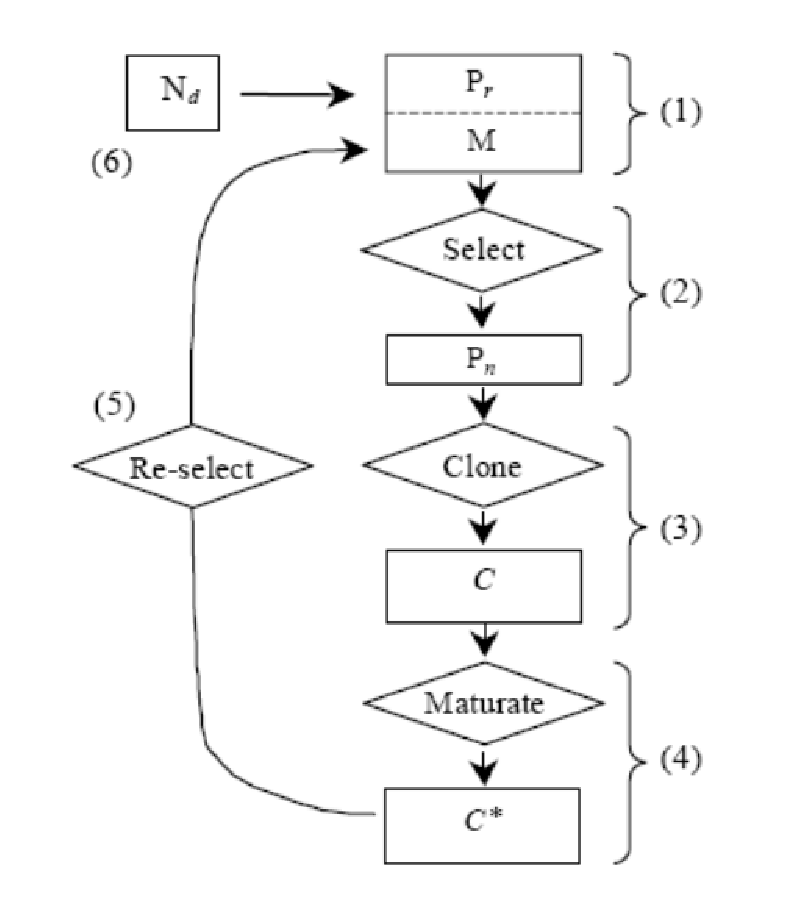
\includegraphics[width=0.5\textwidth]{img/algoritmo}
\end{center}
\caption{Diagrama del algoritmo de la selección clonal}
\label{fig:algoritmo}
\end{figure}

Siendo la explicación de los pasos de la figura~\ref{fig:algoritmo} la siguiente:
\begin{enumerate}
    \item Generar un conjunto (P) de soluciones candidatas, compuesto de células de memoria (M) añadidas a la población restante (Pr), teniendo entonces $P = Pr + M$
    \item Determinar los $n$ mejores individuos (Pn) de la población (P), basado en una medida de afinidad.
    \item Clonar (reproducir) estos $n$ mejores individuos de la población proporcional a su fitness, dando origen a una población temporal de clones (C).
    \item Someter la población de clones a un esquema de hiper-mutación (inversamente proporcional a la afinidad del anticuerpo). Una población de anticuerpos maduros es generada (C*).
    \item Seleccionar nuevamente los mejores individuos de (C*) para componer el conjunto de memoria. (Algunos reemplazos desde (C*) a (P), debido a la mejora)
    \item Reemplazar los $d$ anticuerpos con menor afinidad de la población, manteniendo la diversidad.
\end{enumerate}



\subsection{Estado del Arte Técnica}
\label{sec:estadoArteTecnica}
%Descripción de otras experiencias similares a la que se estudiará.
%Esta sección deberá contener la descripción de experiencias con el mismo problema/técnica
%(las mejores) o para problemas similares que puedan ayudarle como refrencia para su propuesta.

Desde que De Castro et al. publicó su trabajo \emph{`` Learning and optimization using clonal selection principle''}~\cite{decastro},
distintos investigadores se han dedicado a poder utilizar dicha teoría para implementar algoritmos que buscan
optimizar una tarea determinada, de hecho, la mayoría de los trabajos se centran en por ejemplo la \emph{optimización
de funciones}, \emph{optimización multiobjetivo}, sin dejar de lado los problemas típicos de optimización como lo son
\emph{path planning}, \emph{graph coloring}, \emph{vehicle routing}, \emph{entrenamiento de sistemas}, \emph{clasificadores},
\emph{reconocimiento de patrones}, etc, pero la presente sección se centra netamente en problemas abordados que puedan
tener una cierta relación a nivel de modelamiento, objetivos o tratamiento con el problema principal del presente trabajo,
el \emph{Car Sequencing Problem}.\\


% Clonal Selection based Mobile Robot Path Planning

Respecto al área de la robótica, Xuanzi Hu~\cite{robotPlanning} a podido dar un enfoque a las problemáticas relacionadas
con el \emph{Mobile Robot Path Planning}, realizando una comparativa con los algoritmos genéticos, en los cuales queda demostrado
la eficiencia y superioridad de la selección clonal, ya que al ser dos metodologías generacionales, se basan en los mismo principios,
y son fácilmente comparables al momento de realizar un \emph{benchmark} de ambas técnicas con parámetros lo más similar posible.
Una característica especial de la presente implementación son sus operadores inmunes utilizados, en los que están el operador de mutación
que consiste en elegir aleatoriamente un nodo del camino y reemplazarlo por otro nodo que no está en el camino original; el operador
de inserción, que se utiliza para poder reparar los segmentos de un camino infactible, insertando un nodo entre el problema y por último
el operador de supresión, que se aplica a los caminos factibles e infactibles. 

Un punto importante en éste trabajo es que a nivel de programación algorítmica, la selección clonal presenta una superioridad también,
al poder ser un algoritmo mucho más sencillo de  implementar que un algoritmo genético.\\
%%


% Scheduling Aircraft Landing Based on Clonal Selection Algorithm and Receding Horizon Control
Por otro lado Xiaolan Jia et al.~\cite{aircraft} utiliza la selección clonal hibridamente en conjunto con un modelo
de control predictivo llamado \emph{Receding Horizon Control (RHC)} para abordar el conocido problema de \emph{Scheduling Aircraft Landing},
en el cual la selección clonal forma parte del algoritmo RHC, ocupándose de realizar el scheduling propiamente tal.

Detalladamente las dos aproximaciones que plantea el presente trabajo de X. Jia, señala que una selección clonal con restricciones
basado en ``grados de infactibilidad'' (IFD) programa los aviones en el \emph{receding horizon} actual, en cambio
el RHC repite el proceso de optimización usando ``propagación de segmentos excelentes de genes'' (EGSS) hasta que todos los aviones
han aterrizado.

IFD maneja las restricciones de una buena manera y guía el proceso de optimización de manera efectiva,
por otro lado EGSS mejora la velocidad de convergencia del algoritmo, demostrando empíricamente que la aproximación con RHC
soluciona el problema de una manera mas efectiva y rápida.\\
%%


% Clonal Selection Algorithm for Vehicle Routing

Otro problema de optimización conocido como \emph{Vehicle Routing Problem (VRP)} ha sido atacado utilizando la selección clonal
también por varios autores, entre ellos destaca Jacek Dabrowski~\cite{vrp} pues soluciona una pequeña variación del
problema en conjunto llamado \emph{Capacitated Vehicle Routing Problem (CVRP)} en el cual una flota fija de vehículos de repartición
con una capacidad uniforme debe atender la demanda de un cliente determinado para un solo producto de un sólo almacén, cumpliendo
obviamente el mínimo costo de transito. Por lo que la única variación entre CVRP y VRP es que el primero añade la restricción
de que todos los vehículos deben tener una capacidad uniforme de un sólo producto.

Dabrowski señala que la selección clonal es una buena herramienta para la búsqueda de caminos múltiples,
ya que cuando entregamos una instancia del programa se puede un conjunto de soluciones como un conjunto de anticuerpo,
rankeando las soluciones mediante ``operadores de comparación'' y pero que existe un control sobre el ``operador de mutación''
entre los cuales están; EXC, que elige esquinas del camino y las trata de unir; SUM, que intenta concatenar dos rutas sin violar
restricciones; NEW, que construye nuevas ruta utilizando la heurística \emph{greedy} a partir de un vértice aleatorio.

Finalmente el único problema es que el autor señala que sería correcto realizar un benchmark con otras técnicas,
para poder comprobar que tan efectiva es la técnica.\\
%%


% Stretching Technique-based Clonal Selection Algorithm for Flexible Job-shop Scheduling
Como ya se vio anteriormente, en muchas investigaciones se utiliza la mezcla entre la selección clona y otra técnica,
y es el mismo casi que propone Lu Hong~\cite{jobshop} al utilizar una técnica de \emph{Stretching} al resolver
una variación del \emph{Job-shop scheduling problem (JSP)} llamado \emph{Flexible Job-shop Scheduling Problem (FJSP)},
la cual solo posee una mayor disponibilidad de máquinas para realizar las operaciones, es decir, sigue la dinámica
de encontrar una ubicación de cada operación y definir las secuencias de éstas en cada máquina, tratando de utilizar el mínimo
tiempo posible.

La técnica de \emph{stretching} fue propuesta por M. N. Vrahatis~\cite{stretching},
%M. Vrahatis, G. Androulakis and M. Manoussakis, “A new unconstrained optimization method for Imprecise function andgradient values,”
%Journal of Mathematical Analysis and Applications, 1996, pp. 586–607.
y su idea principal es realizar dos etapas de transformación sobre la forma de la función objetivo,
basada en la información de los mínimos locales, es decir, si hay un mínimo se busca realizando un algoritmo
de optimización convencional, y cuando se encuentra, la función objetivo se ``estira'' de acuerdo a unas expresiones determinadas.

Utilizando la función de \emph{stretching} no se cambian los objetivos buscando, pero provee una forma de escape
de los óptimos locales mejorando la convergencia global.

Generalmente luego de los test, STCSA muestra ser mejor que una selección clonal normal,
siendo una excelente aproximación para resolver problemas a larga escala cuando otros algoritmos fallan dando buenas soluciones.\\
%%


% Immune Clonal Selection Algorithm for Hybrid Flow-shop Scheduling Problem
Feng Liu et al.~\cite{flowshop} para poder reducir la complejidad computacional del
\emph{Hybrid Flow-shop Scheduling Problem} utiliza selección clonal.

Éste problema es una aplicación importante en las empresas manufactureras, ya que es un problema NP-completo,
y actualmente las tecnologías de optimización y algunas heurísticas como \emph{branch and bound}, \emph{genetic algorithm}
han sido utilizadas pero sin tanto éxito, ya que tienen distintos inconvenientes al momento de trabajar con problemas
de alto tamaño.

Liu realiza ésta elección, pues la selección clonal propone mecanismos especiales como la habilidad de mantener la diversidad
de los anticuerpos, mecanismos de auto-adaptación y funciones de memoria. Además para mejorar la exploración y explotación
se agrupan estrategias y operadores de multi-mutación (mutación clonal, cruzamiento clonal y selección clonal).\\
%%


% Computer Experiments with a Parallel Clonal Selection Algorithm for the Graph Coloring Problem
Finalmente, existen trabajos dignos de destacar, como la aproximación que entrega Jacek Dabrowski~\cite{graph}
al realizar experimentos con selección clonal pero utilizando conceptos de paralelismo para un problema básico como lo es
el \emph{Graph Coloring Problem}, comparandolo contra un algoritmo \emph{Tabu search} en paralelo.

Los anticuerpos son inicializados utilizando una asignación aleatorias de colores o utilizando una heurística \emph{greedy},
por otro lado, la selección clonal se enfoca a minimizar la función objetivo, siendo ésta el numero de conflictos de colores.

El mecanismo de hiper-mutación cambia la asignación de colores a los vértices del gráfico.

Para mejorar el desempeño de la versión paralela que se ha creado se utilizada el modelo de ``isla'' (asincrónico),
donde cada procesador trabaja con su propio conjunto de anticuerpos.

Lo llamativo surge al existir mecanismos de ``migración'' que permite un intercambio de conocimiento entre los 
distintos procesos, los cuales son elegidos mediante una ``selección de torneo''.

Por lo tanto la selección clonal se sobrepone a \emph{Tabu search} en todas las instancias,
llegando a la conclusión que aunque no posea un operador de cruzamiento, la selección clonal
es una forma fácil de implementar un algoritmo de optimización.
%%


Finalmente los algoritmos inmunes, en especial los algoritmos de ``selección clonal'' suelen ser una buena aproximación
para poder solucionar problemas de optimización y gracias a los estudios analizados en el estado del arte del problema,
podemos decir que es una buena solución para el ``Car Sequencing Problem''.



\section{Bibliografía}
%Se debe referenciar todo paper citado. En caso de referenciar páginas web, debe incluir fecha.
\bibliography{informe}
\end{document} 
